\subsection{Initial Architecture Design}
At the beginning of the project, the model-view-controller architecture has been chosen to be the basis for the TDA. For this, the project is divided into three different layers, each responsible for a specific functionality. In particular, the business logic is separated from the control and presentation layer. This follows the principle of separation of concerns.

The model-view-controller pattern is defined as a compound pattern. This means that it is a combination of several other design patterns that work together. As the name predicts, it consists of a model, view and controller, which all have different responsibilities. The view is responsible for displaying information and for allowing interaction with the user. The model holds the program's data and executes all related computations. It is the representation of the business logic. Finally, the controller works close with the view and functions as a translator for the interaction between the previously mentioned components. View and controller together build the user interface.
While the model can function on its own, view and controller depend on the existence of a model. This makes the user interface easily changeable or even exchangeable as a whole, without touching the logic at all. In other words, the proposed architecture is also designed for change. Additionally, it is possible to implement multiple views next to each other, all relying on the same underlying logic. The preferred view can then even be displayed at run time and for example based on the machine or device it is being executed on.

Since the TDA shall display all the information in an adequate graphical user interface, this approach seemed to fulfill the criteria and fit our needs. Although there were no concrete plans for implementing an additional user interface, it is always a good practice to be prepared for similar requests that arise later in the project phase. Figure \ref{MVCdiagram} shows the high level architecture diagram of this approach.

\begin{figure}
\begin{center}
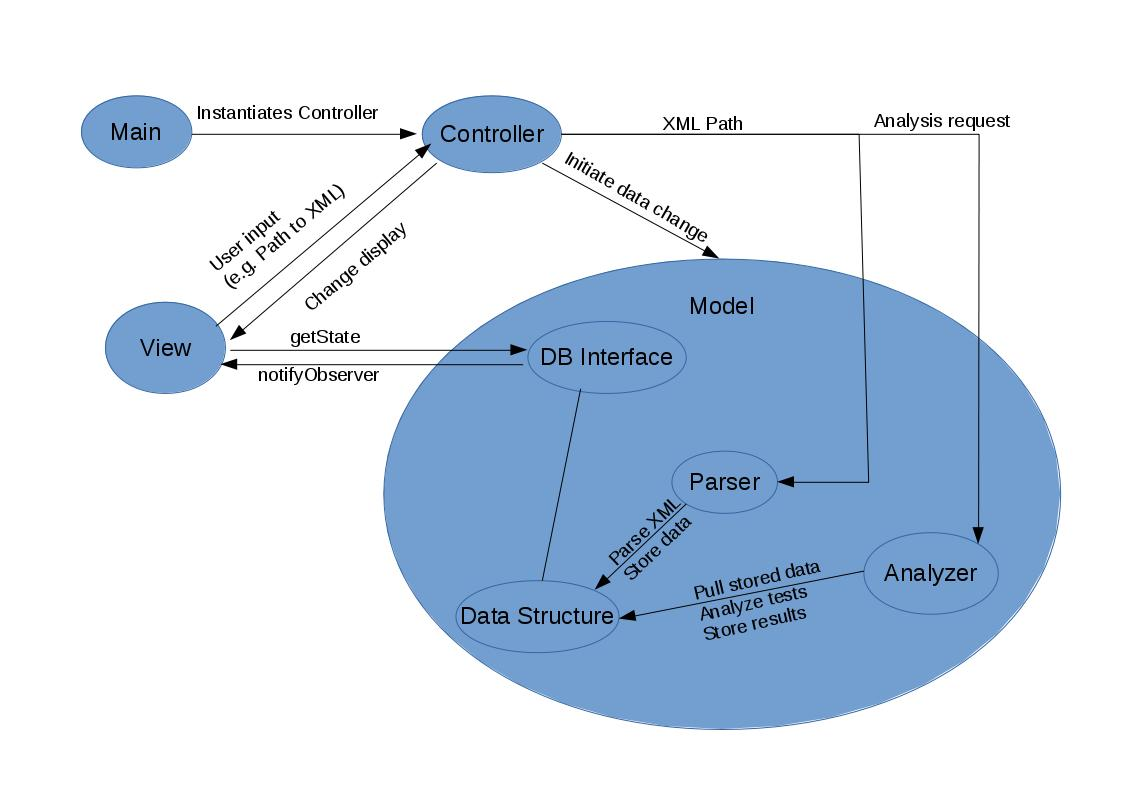
\includegraphics[scale=0.35]{pics/Architecture_diagram.jpg}
\caption{MVC Architecture Diagram}
\label{MVCdiagram}
\end{center}
\end{figure}

Also very early in the project development, we discussed how the given XML-files shall be read and whether they shall be processed and stored internally for later, faster processing. Database approaches were discussed and compared to directly loading the information in an internal infrastructure. A detailed description of this process and the final results can be found in section~\ref{sec:data_structures}.
The selected data structure and its location also have a big influence on the selected architecture and the overall class interaction. With the current approach, this clearly was a part of the model.

After other components like the parser and the analyzer were addressed in later project development, the model steadily increased in size and with it in complexity. Other design patterns and architectures were needed, in order to maintain the highly flexible and clearly structured code that we strive to achieve. That's why we changed the high-level architecture, as described in detail in the following paragraph, and used the previously explained model-view-controller pattern only as a subsystem for the new architecture.


\subsection{Final Architecture Design}
The high level architecture of the TDA now follows the repository architecture. This design is defined by one central entity and different subsystems that are connected directly to the named system. The central entity hereby usually functions as a data storage. In the following, the advantages and disadvantages are being weighed against each other and it is concluded why the introduced architecture is a good fit to our needs.

The repository architecture in general is designed for change. Having different subsystems for different functionality allows for exchangeability and therefore flexibility in the later software development and maintenance. Also adding or removing subsystems can easily be done. Furthermore, the central data storage allows for convenient and consistent data management. Data is only stored at one position and is not hold by any subsystem. This means that changes to the data system are automatically propagated to other components through the shared repository. Subsystems therefore also don't need to worry about how and where the given information is processed and used. They just have to follow the given restrictions on accepted data types.

This also names one of the challenges of the repository architecture. All components need to agree on a certain standard of communication and use the same data types to be compatible. Additionally, one single access point also introduces a single point of failure. It therefore is extremely important that the used system is failure robust and stable over time. The repository should also be able to handle multiple requests at the same time and manage resources efficiently. Since all other systems depend on it, a slowdown would affect the whole project. Finally, the distribution of the repository across many different machines may cause some additional challenges.

It can be concluded that the introduces repository architecture simplifies the access and management of the data in a project significantly. This comes with some restrictions in terms of the communication and data types. Therefore, the proposed architecture is often only a solution for relatively small and structured systems [FSE – V14, p26].

The Test Data Analyzer represents such a small and structured system. Also the project has a limited scope and therefore the final product will remain rather small. Lastly, the repository is well suited for projects with a database. Since the TDA stores data internally, this is fitting too. To concluded, the TDA is benefiting from all of the repository architecture's advantages while limiting the disadvantages to a minimum. Therefore, the proposed architecture is well suited as a high level architecture for the overall project.

While the internal data structure represents the repository, the other components act as its subsystems. These include the user interface, the parser and the analyzer.

To make the repository even more omnipresent, we implemented it as Singleton. This creational design pattern allows to instantiate one and only one instance of the class. Additionally, every other class can access this single instance by using a special static getter method. This ensures that every class can easily access all of the repository's data and methods, without actually holding an own reference. Not only does this prevent unnecessary reference passing, it also ensures data consistency by making sure that no other class creates or holds a different instance of the repository. Figure \ref{RepoDiagram} shows the high level architecture of this approach.

\begin{figure}[h]
\begin{center}
\includegraphics[scale=0.6]{pics/repository_architecture.png}
\caption{Repository Architecture Diagram}
\label{RepoDiagram}
\end{center}
\end{figure}

\subsection{Object Oriented Design Principles}

This section summarizes all further design patterns and principles that were applied over the course of this project and taught in the Software Engineering lecture.

A set of important principles, that also includes many other patterns and summarize their main ideas, are the so called \textbf{S.O.L.I.D. principles}. In the following, every principle is explained and displayed how it has affected our design decisions.

%[Based on http://butunclebob.com/ArticleS.UncleBob.PrinciplesOfOod]

\paragraph{Single Responsibility Principle (SRP):}
The SRP states that every responsibility should be in a separate class. This principle also includes the principle of separation of concerns, which has been one of our major objectives. It was taken into account at any time during the development process and led to smaller and more thought through classes with clear responsibilities. As already mentioned previously, also the used architectures rely on this idea.
\paragraph{The Open-Closed Principle (OCP):}
``A class should be open for extension, but closed for modification'' [B. Meyer]\\
This means that a class' behavior should be able to be extended, without changing it. Usually, this is achieved by using abstract classes and well-defined class descriptions (interfaces). The latter was also a crucial part of our project and will be discussed in the following principles.
\paragraph{The Liskov Substitution Principle (LSP):}
We always tried to program to an interface, not an implementation. For example, both parser and analyzer relied on an interface. Using interfaces brought many benefits, including the already mentioned exchangeability. To make this possible, subtypes must be substitutable for their base types. This is exactly what the Liskov Substitution Principle stands for. 
\paragraph{The Interface Segregation Principle (ISP):}
Closely related to the previous principle is the ISP. It describes that the dependency between classes should depend on the smallest possible interface. To look at it from another perspective, it also means to avoid "fat" or "polluted" interfaces. Such an interface can be broken up into groups of member functions. Each group serves a different set of clients. We always prevented this by making our interfaces as small and cohesive as possible. The size of the project probably also helped maintaining this property.
\paragraph{The Dependency Inversion Principle (DIP):}
The principle can best be summarized in these two aspects:
\begin{enumerate}
\item High level modules should not depend upon low level modules. Both should depend upon abstractions.
\item Abstractions should not depend upon details. Details should depend upon abstractions.
\end{enumerate}
These two properties are essential in creating object oriented software that is resilient to change. Since the abstractions and details are all isolated from each other, the code is also much easier to maintain. It also prevents tight coupling and difficult class dependencies. Therefore, the whole system architecture was designed with the dependency inversion principle in mind.

\subsection{Data Structure}\label{sec:data_structures}

Since the application's main task is to read and evaluate information stored in XML-files, it was crucial for the project to discuss how this data will be processed and how it then later can again be accessed. We soon concluded that we want to save the parsed data in an own internal storage system to make it available for fast access at later point, without the need of parsing any further information. This also correlated with our client needs, who made clear that he would rather wait longer in the beginning than while using the program.\\
We first thought about storing the information in an SQL database and therefore looked up possible ways of implementing this without generating too much overhead. We soon realized that without the use of external libraries this task would require too much of our precious time, since we all were no experts on implementing databases from scratch in java.\\
Instead, we set up an internal data structure that parsed all information from the XML-files into different, corresponding classes. This infrastructure allows to lookup information from any TestRun, TestedClass or UnitTest. And since the access point to the data structure is represented by our repository, this information can be accessed anytime from anywhere in the whole project.\\




